% !TEX program = xelatex
% !TEX encoding = UTF-8 Unicode
\documentclass[13pt,a4paper,oneside]{report}

\usepackage{fontspec}
\usepackage{polyglossia}
\setmainlanguage{vietnamese}
\setotherlanguage{english}
\setmainfont{lmroman10-regular.otf}[
  BoldFont=lmroman10-bold.otf,
  ItalicFont=lmroman10-italic.otf,
  BoldItalicFont=lmroman10-bolditalic.otf]
\usepackage{geometry}
\geometry{a4paper,left=3cm,right=2cm,top=2cm,bottom=2cm}
\usepackage{setspace}
\onehalfspacing
\usepackage{amsmath,amssymb}
\usepackage{graphicx}
\usepackage{booktabs}
\usepackage{tabularx}
\usepackage{float}
\usepackage{caption}
\usepackage{siunitx}
\sisetup{group-separator={,},group-minimum-digits=4,detect-all}
\captionsetup{font=small,labelfont=bf,labelsep=endash}
\usepackage[table]{xcolor}
\usepackage{tikz}
\usetikzlibrary{arrows.meta,positioning,fit,backgrounds}
\usepackage[unicode,hidelinks]{hyperref}

\urlstyle{tt}
\def\UrlBreaks{\do\/\do\_\do\.\do\-\do\,\do\{\do\}}
\Urlmuskip=0mu plus 1mu\relax

\usepackage{titlesec}
\titleformat{\chapter}[display]
  {\normalfont\Large\bfseries\centering}{\chaptertitlename\ \thechapter}{12pt}{\LARGE}
\titlespacing*{\chapter}{0pt}{10pt}{24pt}
\setlength{\parindent}{1.2em}
\setlength{\emergencystretch}{3em}

\begin{document}
\sloppy

\begin{titlepage}
\centering
{\large BỘ GIÁO DỤC VÀ ĐÀO TẠO\par}
{\large TRƯỜNG ĐẠI HỌC FPT --- VIỆN QUẢN TRỊ \& CÔNG NGHỆ (FSB)\par}
\vfill
{\LARGE\bfseries TÁI LẬP VÀ ĐÁNH GIÁ CÓ KIỂM SOÁT CRYPTOMAMBA\\[6pt]
CHO DỰ BÁO GIÁ BITCOIN NGÀY KẾ TIẾP\par}
\vspace{10pt}
{\large LUẬN VĂN THẠC SĨ\par}
\vfill
\begin{flushright}
\begin{tabular}{@{}ll@{}}
Học viên thực hiện: & Trần Huỳnh Anh Hiếu \\
Giảng viên hướng dẫn: & Nguyễn Duy Nghiêm \\
\end{tabular}
\end{flushright}
\vfill
{\large Việt Nam --- 2026\par}
\end{titlepage}

\pagenumbering{roman}

\chapter*{Tóm tắt}
\addcontentsline{toc}{chapter}{Tóm tắt}
Luận văn tái lập CryptoMamba-v (CM-v) cho dự báo giá đóng cửa Bitcoin ngày kế tiếp và đánh giá lại
các kết luận của bài báo gốc. Trên giao thức 350 ngày, RMSE, MAE và MAPE của checkpoint tái lập
chênh lần lượt \num{0.892}\%, \num{1.057}\% và \num{0.718}\% so với số liệu công bố. Đánh giá có
kiểm soát tiếp theo so sánh CM-v, mô hình thử nghiệm CMamba-T/S5-Full và naive persistence trên cùng
304 ngày validation và 304 ngày test. Trên test, RMSE lần lượt là \num{1703.51}, \num{1660.83} và
\num{1657.55}; kiểm định Diebold--Mariano và khoảng bootstrap theo khối không xác nhận ưu thế RMSE
của S5-Full so với CM-v. CM-v đạt directional accuracy \num{57.57}\%; kiểm định McNemar không xác
nhận khác biệt hướng giữa hai mô hình. Persistence được loại khỏi phép đo hướng vì chỉ giữ nguyên
mức giá hiện tại.
Kết luận cặp về RMSE và hướng không đổi với các độ dài khối bootstrap
$L=\num{5},\num{7},\num{14}$.

Luận văn bổ sung hai lớp đánh giá. Thứ nhất, replay không phí giữ nguyên thuật toán của bài báo để
đối chiếu checkpoint. Thứ hai, một engine self-financing tách biệt tính phí trên giá trị giao dịch,
giới hạn tổng mức phơi nhiễm và đối soát vốn cuối kỳ. Buy-and-hold cao hơn mọi chiến lược dựa trên
dự báo ở cả ba mức phí; tại \num{0.2}\% trên test, số dư là \$\num{158.09}. S5-Full dùng
\num{57249} tham số so với
\num{136952} của CM-v; mô hình có RMSE thấp hơn CM-v trên validation và test nhưng không vượt
persistence. Cuối cùng, một Console năm màn hình trình bày dữ liệu, đánh giá, suy luận checkpoint,
giao dịch và kiến trúc; luồng chính cho phép tải dữ liệu mới, chọn checkpoint CM-v hoặc S5-Full và
dự báo mà không cần huấn luyện lại.

Về phạm vi ứng dụng, đề tài được đặt trong bối cảnh Việt Nam thí điểm thị trường tài sản mã hóa theo
Nghị quyết 05/2025/NQ-CP; luận văn không thực hiện phân tích pháp lý hoặc đưa ra tư vấn đầu tư.

\vspace{6pt}
\noindent\textbf{Từ khoá:} \textit{Bitcoin, dự báo chuỗi thời gian, Mamba, tái lập nghiên cứu,
naive persistence, kiểm định dự báo, self-financing backtest, thị trường tài sản mã hóa Việt Nam.}

\tableofcontents
\listoffigures
\addcontentsline{toc}{chapter}{Danh mục hình}
\listoftables
\addcontentsline{toc}{chapter}{Danh mục bảng}

\chapter*{Danh mục từ viết tắt}
\addcontentsline{toc}{chapter}{Danh mục từ viết tắt}
\renewcommand{\arraystretch}{1.22}
\begin{tabularx}{\linewidth}{@{}lX@{}}
\toprule
\textbf{Viết tắt} & \textbf{Diễn giải} \\
\midrule
API & Application Programming Interface \\
BTC & Bitcoin \\
CM-v & CryptoMamba-v, biến thể dùng khối lượng \\
DM & Diebold--Mariano \\
HAC & Heteroskedasticity and Autocorrelation Consistent \\
MAE & Mean Absolute Error \\
MAPE & Mean Absolute Percentage Error \\
MDD & Maximum Drawdown \\
OHLCV & Open--High--Low--Close--Volume \\
RMSE & Root Mean Square Error \\
ROI & Return on Investment \\
SSM & State Space Model \\
\bottomrule
\end{tabularx}
\renewcommand{\arraystretch}{1.0}

\cleardoublepage
\pagenumbering{arabic}

% ---------------------------------------------------------------------
\chapter{Giới thiệu}\label{chap:intro}

\section{Bối cảnh nghiên cứu}\label{sec:motivation}
Dự báo giá Bitcoin ngày kế tiếp là một bài toán khó vì chuỗi giá phi dừng, biến động mạnh và có mức
tự tương quan rất cao ở thang giá tuyệt đối. Trong bối cảnh đó, sai số thấp chưa đủ chứng minh mô
hình khai thác được thông tin mới: phép dự báo đơn giản giữ nguyên giá đóng cửa hiện tại thường đã
là một đối chứng mạnh.

Bài báo CryptoMamba \cite{cryptomamba} áp dụng Mamba \cite{mamba} cho dữ liệu BTC-USD ngày và báo
cáo CryptoMamba-v tốt hơn LSTM-v, Bi-LSTM-v, GRU-v, iTransformer-v và S-Mamba-v trên RMSE, MAE,
MAPE. Bài báo cũng đưa dự báo vào ba thuật toán giao dịch. Tuy nhiên, bảng công bố chỉ chứa chỉ số
tổng hợp; không có chuỗi sai số theo ngày để kiểm định cặp, và phần giao dịch chưa mô hình hoá phí
giao dịch theo một sổ cái self-financing. Luận văn tập trung vào khoảng trống đánh giá này, đồng
thời xây dựng một biến thể nhẹ và một hệ thống minh hoạ có thể kiểm tra trực tiếp.

\section{Mục tiêu và câu hỏi nghiên cứu}\label{sec:rq}
Mục tiêu là tái lập CM-v, đánh giá dự báo và giao dịch trên các giao thức xác định, thử nghiệm một
biến thể nhẹ, và trực quan hóa toàn bộ quy trình bằng một Console năm màn hình. Bốn câu hỏi nghiên
cứu là:
\begin{itemize}
\item \textbf{RQ1 -- Tái lập.} CM-v và replay giao dịch từ mã nguồn công bố có tái tạo được các kết
quả của bài báo ở mức độ nào?
\item \textbf{RQ2 -- Đánh giá.} Trên cùng các ngày mục tiêu, CM-v, S5-Full và naive persistence khác
nhau như thế nào về sai số, hướng dự báo và ý nghĩa thống kê?
\item \textbf{RQ3 -- Giao dịch.} Kết quả dự báo chuyển thành kết quả giao dịch như thế nào khi tách
replay của bài báo khỏi một engine corrected self-financing có phí?
\item \textbf{RQ4 -- Mô hình.} S5-Full có tạo ra một mô hình nhẹ hơn với kết quả thực nghiệm đủ để
khẳng định ưu thế dự báo hay không?
\end{itemize}

\section{Phạm vi}\label{sec:scope}
Nghiên cứu sử dụng một tài sản BTC-USD, nến ngày OHLCV, dự báo một bước và các khoảng thời gian của
bài báo. Đánh giá cục bộ chỉ gồm ba mô hình có dự báo theo ngày và có thể căn chính xác: CM-v tái
lập, S5-Full và naive persistence. Các hàng mô hình khác chỉ xuất hiện trong bảng tham chiếu
\emph{Paper-reported}; chúng không được đưa vào kiểm định cặp cục bộ.

Về bối cảnh ứng dụng, đề tài được đặt trong giai đoạn Việt Nam triển khai thí điểm thị trường tài sản
mã hóa theo Nghị quyết 05/2025/NQ-CP, có hiệu lực từ ngày 09-09-2025 với thời gian thí điểm 5 năm
\cite{nq05}. Nghị quyết chỉ xác định bối cảnh ứng dụng; phạm vi kỹ thuật không mở rộng sang phân tích
pháp lý, đánh giá tuân thủ hoặc tư vấn đầu tư.

Luồng sử dụng chính là dữ liệu bài báo hoặc CSV mới $\to$ kiểm tra dữ liệu $\to$ chọn checkpoint
CM-v/S5-Full $\to$ dự báo giá ngày kế tiếp. Historical replay được giữ để minh hoạ quá khứ. Suy
luận qua HTTP bên ngoài là chế độ tuỳ chọn, không phải điều kiện để sử dụng hệ thống. Sản phẩm là
prototype nghiên cứu, không phải hệ thống tư vấn hay thực thi giao dịch.

\section{Đóng góp}\label{sec:contrib}
\begin{enumerate}
\item \textbf{Reproduction.} Tái lập CM-v, đối chiếu checkpoint chính thức và checkpoint tái lập,
đồng thời kiểm tra replay giao dịch của bài báo.
\item \textbf{Evaluation.} Bổ sung naive persistence, so sánh các mô hình trên cùng ngày mục tiêu và
kiểm định sự khác biệt bằng DM/Wilcoxon.
Độ bất định, biến thiên theo thời gian và độ nhạy theo phí được đánh giá bằng bootstrap theo khối,
hai nửa thời gian và ba mức phí cố định.
\item \textbf{Model.} Cài đặt và đánh giá S5-Full, một thí nghiệm CMamba-T nhẹ; kết quả dương, âm và
không có ý nghĩa thống kê đều được báo theo đúng split.
\item \textbf{System.} Xây dựng Console năm màn hình để trình bày data $\to$ prediction $\to$
evaluation $\to$ trading $\to$ architecture, với suy luận trực tiếp từ hai checkpoint cục bộ.
\end{enumerate}

% ---------------------------------------------------------------------
\chapter{Nền tảng và công trình liên quan}\label{chap:background}

\section{Dự báo chuỗi thời gian và đường cơ sở persistence}\label{sec:persistence}
Với dự báo một bước, naive persistence đặt
\begin{equation}\label{eq:persistence}
\widehat{y}_{t+1}=y_t,
\end{equation}
trong đó $y_t$ là giá đóng cửa hiện tại. Baseline này không có tham số và không phát hướng tăng hoặc
giảm. Nó phù hợp để kiểm tra liệu mô hình học sâu có cải thiện so với việc giữ nguyên quan sát gần
nhất hay chỉ tái tạo mức giá hiện tại.

iTransformer đảo cách token hoá phổ biến của Transformer để mô hình hoá quan hệ giữa các biến
\cite{itransformer}. S-Mamba dùng Mamba hai chiều cho quan hệ liên biến và mạng feed-forward cho
quan hệ theo thời gian \cite{smamba}. Hai kiến trúc này nằm trong bảng so sánh của CryptoMamba,
nhưng luận văn chỉ dùng các con số tổng hợp do bài báo công bố vì không có chuỗi dự báo theo ngày.

\section{State Space Model và Mamba}\label{sec:mamba}
Một SSM tuyến tính mô tả trạng thái ẩn $h_t$ và đầu ra $z_t$ theo
\begin{equation}\label{eq:ssm}
h_t=\bar{A}h_{t-1}+\bar{B}x_t, \qquad z_t=Ch_t.
\end{equation}
Mamba làm các tham số chuyển trạng thái phụ thuộc đầu vào, nhờ đó thông tin được giữ hoặc loại theo
từng phần tử của chuỗi; thuật toán có độ phức tạp tuyến tính theo độ dài chuỗi \cite{mamba}. Ý nghĩa
của một phép quét vì vậy phụ thuộc trực tiếp vào trục được đưa vào làm trục chuỗi.

\section{CryptoMamba-v: mô tả công bố và đường chạy mã nguồn}\label{sec:cmv}
Bài báo mô tả CryptoMamba bằng các C-Block nối tiếp và một Merge block. Mỗi C-Block gồm nhiều
CMBlock và một MLP; đầu vào là một cửa sổ các quan sát quá khứ, đầu ra là giá đóng cửa ngày kế tiếp
\cite{cryptomamba}. Hình~\ref{fig:paper-source-architecture} tách phần mô tả khái niệm này khỏi điều
có thể xác nhận từ mã nguồn phát hành.

\begin{figure}[H]
\centering
\resizebox{\linewidth}{!}{% Paper description versus the released CM-v execution path.
\begingroup
\definecolor{archBlue}{HTML}{E8F0FB}
\definecolor{archBlueEdge}{HTML}{5A7FBE}
\definecolor{archGreen}{HTML}{E4F3EC}
\definecolor{archGreenEdge}{HTML}{418B72}
\definecolor{archGold}{HTML}{FFF1CF}
\definecolor{archGoldEdge}{HTML}{B4882C}
\definecolor{archGrey}{HTML}{F5F7F9}
\definecolor{archGreyEdge}{HTML}{AAB4BD}
\definecolor{archInk}{HTML}{263238}

\tikzset{
  input/.style={draw=archBlueEdge, fill=archBlue, rounded corners=3pt,
    minimum width=2.9cm, minimum height=1.05cm, align=center, inner sep=4pt,
    font=\sffamily\small\bfseries, text=archInk},
  process/.style={draw=archGreenEdge, fill=archGreen, rounded corners=3pt,
    minimum width=2.6cm, minimum height=1.05cm, align=center, inner sep=4pt,
    font=\sffamily\small\bfseries, text=archInk},
  repeat/.style={draw=archGreenEdge, fill=archGreen, rounded corners=3pt,
    minimum width=1.75cm, minimum height=1.05cm, align=center, inner sep=3pt,
    font=\sffamily\small\bfseries, text=archInk},
  stage/.style={repeat, minimum width=2.45cm, minimum height=1.30cm},
  head/.style={draw=archGoldEdge, fill=archGold, rounded corners=3pt,
    minimum width=2.25cm, minimum height=1.05cm, align=center, inner sep=4pt,
    font=\sffamily\small\bfseries, text=archInk},
  output/.style={draw=archBlueEdge, fill=archBlue, rounded corners=3pt,
    minimum width=2.2cm, minimum height=1.05cm, align=center, inner sep=4pt,
    font=\sffamily\small\bfseries, text=archInk},
  group/.style={draw=archGreenEdge, fill=archGreen!38, dashed, rounded corners=5pt,
    line width=0.75pt, inner xsep=5pt, inner ysep=5pt},
  lane/.style={draw=archGreyEdge, fill=archGrey, rounded corners=6pt,
    line width=0.65pt, inner xsep=7pt, inner ysep=8pt},
  note/.style={font=\sffamily\scriptsize, text=archInk, align=center},
  title/.style={font=\sffamily\small\bfseries, text=archInk, align=left},
  flow/.style={-{Stealth[scale=1.2]}, draw=archInk, line width=0.85pt}
}

\begin{tikzpicture}[font=\sffamily\small, node distance=0.6cm and 0.8cm]
  \node[input] (paperInput)
    {14-day input\\{\scriptsize\mdseries OHLCV + Timestamp}};
  \node[repeat, right=of paperInput] (paperBlockOne)
    {C-Block 1};
  \node[repeat, right=of paperBlockOne] (paperBlockTwo)
    {C-Block 2};
  \node[repeat, right=of paperBlockTwo] (paperBlockThree)
    {C-Block 3};
  \node[head, right=of paperBlockThree] (paperMerge)
    {Merge};
  \node[output, right=of paperMerge] (paperOutput)
    {Next Close};

  \node[note, above=0.18cm of paperBlockTwo] (paperGroupTitle)
    {C-Blocks};
  \node[title, above=0.34cm of paperInput.north west, anchor=south west] (paperTitle)
    {Paper description\\[-1pt]{\scriptsize\mdseries Sections 4.1--5.1 and Figure 1}};

  \draw[flow] (paperInput) -- (paperBlockOne);
  \draw[flow] (paperBlockOne) -- (paperBlockTwo);
  \draw[flow] (paperBlockTwo) -- (paperBlockThree);
  \draw[flow] (paperBlockThree) -- (paperMerge);
  \draw[flow] (paperMerge) -- (paperOutput);

  \node[input, below=3.0cm of paperInput] (sourceInput)
    {Tensor\\$[B,6,14]$};
  \node[stage, right=of sourceInput] (sourceStageOne)
    {Stage 1\\{\scriptsize\mdseries 4 CMBlocks}\\{\scriptsize\mdseries Linear 14 $\to$ 16}};
  \node[stage, right=of sourceStageOne] (sourceStageTwo)
    {Stage 2\\{\scriptsize\mdseries 4 CMBlocks}\\{\scriptsize\mdseries Linear 16 $\to$ 32}};
  \node[stage, right=of sourceStageTwo] (sourceStageThree)
    {Stage 3\\{\scriptsize\mdseries 4 CMBlocks}\\{\scriptsize\mdseries Linear 32 $\to$ 1}};
  \node[head, right=of sourceStageThree] (sourceHead)
    {Permute +\\{\scriptsize\mdseries Linear 6 $\to$ 1}};
  \node[output, right=of sourceHead] (sourceOutput)
    {Next Close};

  \node[note, above=0.18cm of sourceStageTwo] (sourceGroupTitle)
    {3 stages; scan over 6 feature tokens};
  \node[title, above=0.34cm of sourceInput.north west, anchor=south west] (sourceTitle)
    {Released implementation\\[-1pt]{\scriptsize\mdseries \texttt{CMamba.forward}}};

  \draw[flow] (sourceInput) -- (sourceStageOne);
  \draw[flow] (sourceStageOne) -- (sourceStageTwo);
  \draw[flow] (sourceStageTwo) -- (sourceStageThree);
  \draw[flow] (sourceStageThree) -- (sourceHead);
  \draw[flow] (sourceHead) -- (sourceOutput);

  \begin{scope}[on background layer]
    \node[lane,
      fit=(paperTitle)(paperInput)(paperBlockOne)(paperBlockThree)(paperMerge)(paperOutput)
          (paperGroupTitle)] {};
    \node[group, fit=(paperBlockOne)(paperBlockThree)(paperGroupTitle)] {};
    \node[lane,
      fit=(sourceTitle)(sourceInput)(sourceStageOne)(sourceStageThree)
          (sourceHead)(sourceOutput)(sourceGroupTitle)] {};
    \node[group, fit=(sourceStageOne)(sourceStageThree)(sourceGroupTitle)] {};
  \end{scope}
\end{tikzpicture}
\endgroup
}
\caption[Paper diagram and released CM-v execution]{Paper-described pipeline versus the
source-derived CM-v execution path. The upper row combines the data/input description in Sections
4.1 and 5.1 with the architecture in Section 4.2 and Figure 1 of CryptoMamba; the lower row is
derived from the released \texttt{CMamba.forward} implementation.}
\label{fig:paper-source-architecture}
\end{figure}

Trong mã nguồn, CM-v nhận tensor $[B,6,14]$. Khối Mamba nhận 6 token đặc trưng với độ rộng 14; ba
tầng linear đổi độ rộng $14\to16\to32\to1$, mỗi tầng chứa bốn CMBlock. Head cuối permute tensor và
dùng Linear $6\to1$. Cấu hình thực thi có \num{136952} tham số. Nhận xét này chỉ mô tả đường chạy
đã phát hành; sơ đồ khái niệm trong bài báo không biểu diễn chi tiết trục tensor.

\section{So sánh độ chính xác dự báo}\label{sec:stats-background}
Diebold--Mariano (DM) kiểm tra giả thuyết không về độ chính xác bằng nhau của hai dự báo
\cite{dm}. Luận văn dùng sai biệt tổn thất bình phương
$d_t=e_{A,t}^{2}-e_{B,t}^{2}$ và ước lượng phương sai HAC với lag 1 theo Newey--West
\cite{neweywest}. Wilcoxon signed-rank \cite{wilcoxon} được áp dụng độc lập trên sai biệt sai số
tuyệt đối $|e_{A,t}|-|e_{B,t}|$. Hai kiểm định trả lời hai câu hỏi khác nhau nên không được trình
bày như cùng một phép đo.

% ---------------------------------------------------------------------
\chapter{Phương pháp nghiên cứu}\label{chap:method}

\section{Dữ liệu và chia tập theo thời gian}\label{sec:data}
Dữ liệu BTC-USD ngày được lấy theo giao thức của bài báo, từ ngày 17-09-2018 đến 17-09-2024. Các
trường đầu vào là Timestamp, Open, High, Low, Close và Volume. Chia tập giữ nguyên thứ tự thời gian
và không xáo trộn (Bảng~\ref{tab:splits}).

\begin{table}[htbp]
\centering
\caption{Chia tập theo giao thức CryptoMamba.}
\label{tab:splits}
\begin{tabularx}{\linewidth}{@{}lXX@{}}
\toprule
\textbf{Tập} & \textbf{Khoảng thời gian} & \textbf{Vai trò} \\
\midrule
Train & 17-09-2018 đến trước 17-09-2022 & Ước lượng tham số \\
Validation & 17-09-2022 đến trước 17-09-2023 & Chọn checkpoint \\
Test & 17-09-2023 đến trước 17-09-2024 & Đánh giá cuối \\
\bottomrule
\end{tabularx}
\end{table}

CM-v dùng cửa sổ 14 ngày; S5-Full dùng cửa sổ 60 ngày. Để so sánh cặp, luận văn lấy giao các ngày
mục tiêu mà cả ba mô hình đều có dự báo: 304 ngày validation (16-11-2022 đến 15-09-2023) và 304
ngày test (16-11-2023 đến 14-09-2024). Mọi bảng cục bộ, kiểm định và corrected backtest đều dùng
đúng các giao này. Bảng tổng hợp 350 ngày theo giao thức giấy gốc chỉ phục vụ RQ1 và không được trộn
với phép kiểm định 304 ngày.

\section{Mô hình và checkpoint}\label{sec:model-contracts}
Cả hai mô hình được đánh giá trên cùng biến mục tiêu: giá Close gốc của ngày kế tiếp. Đặc tả đầu vào
và đầu ra khác nhau như tóm tắt trong Bảng~\ref{tab:model-contracts}.

\begin{table}[H]
\centering
\caption{Hợp đồng đầu vào, tiền xử lý và đầu ra của CM-v và S5-Full.}
\label{tab:model-contracts}
{\small
\begin{tabularx}{\linewidth}{@{}lXX@{}}
\toprule
\textbf{Thành phần} & \textbf{CM-v} & \textbf{S5-Full} \\
\midrule
Biến mục tiêu & Close gốc của ngày kế tiếp & Close gốc của ngày kế tiếp \\
Cửa sổ đầu vào & 14 ngày, $[B,6,14]$ & 60 ngày, $[B,5,60]$ \\
Trường đầu vào & Timestamp + OHLCV & OHLCV; không dùng Timestamp \\
Giá đầu vào & Giá gốc & $x/C_t-1$ \\
Volume đầu vào & $\mathrm{Volume}/10^9$ & $\log(1+\mathrm{Volume}/10^9)$ \\
Đầu ra mô hình & Close ngày kế tiếp & Return tương đối $\widehat r_{t+1}$ \\
Dự báo cuối & Đầu ra trực tiếp & $C_t(1+\widehat r_{t+1})$ \\
\bottomrule
\end{tabularx}}
\end{table}

Checkpoint tái lập được dùng để đánh giá và suy luận CM-v. S5-Full là định danh thí nghiệm cục bộ
cho kiến trúc CMamba-T; nó không phải lớp S5 được công bố như một họ SSM độc lập. Bốn CMBlock có
$d_{state}=16$ xử lý chuỗi 60 day-token; biểu diễn ngày gần nhất đi qua LayerNorm và Linear
$32\to1$. Checkpoint seed 23 tại best epoch 321 có \num{57249} tham số.

Hai mô hình vì vậy được chấm trên cùng không gian giá và cùng ngày mục tiêu. Do cửa sổ đầu vào,
tiền xử lý, cách tham số hoá đầu ra và kiến trúc thay đổi đồng thời, đây là so sánh end-to-end giữa
hai model pipeline, không phải một ablation chỉ thay đổi kiến trúc.

Khi suy luận, dữ liệu được kiểm tra và lấy cửa sổ tương ứng với mô hình trước khi nạp checkpoint đã
chọn. Quy trình chỉ dự báo và không cập nhật trọng số.

\section{Độ đo và kiểm định}\label{sec:metrics}
Với $e_t=y_t-\widehat{y}_t$, ba độ đo chính là
\begin{align}
\mathrm{RMSE} &= \sqrt{\frac{1}{n}\sum_{t=1}^{n}e_t^2}, &
\mathrm{MAE} &= \frac{1}{n}\sum_{t=1}^{n}|e_t|, \\
\mathrm{MAPE} &= \frac{100}{n}\sum_{t=1}^{n}\left|\frac{e_t}{y_t}\right|.
\end{align}
Hướng dự báo là dấu của $\widehat{y}_{t+1}-y_t$ và hướng thực là dấu của $y_{t+1}-y_t$.
Directional accuracy chỉ được tính cho mô hình tạo dự báo tăng hoặc giảm; naive persistence không
tham gia phép đo này. Các kiểm định DM và Wilcoxon dùng đúng cặp ngày, hai phía, mức ý nghĩa
$\alpha=0.05$.

Để giữ phụ thuộc chuỗi thời gian, luận văn dùng non-circular moving-block bootstrap
\cite{kunsch1989,buhlmann1999}. Với $n=304$, luận văn cố định
$L=\lceil n^{1/3}\rceil=\num{7}$ như một quy tắc kinh nghiệm cùng bậc $n^{1/3}$, dùng
\num{50000} lần lấy mẫu và seed tính toán bootstrap \num{230813}; seed này khác seed huấn luyện.
Phân tích cặp được lặp tại $L=\num{5}$ và $L=\num{14}$ trong khi giữ nguyên dữ liệu, dự báo,
số lần lấy mẫu và seed tính toán. Ở đây $L$ là độ dài khối bootstrap, không phải cửa sổ đầu vào của
mô hình. $L=\num{7}$ không được xem là tối ưu. Khoảng
percentile 95\% giả định chuỗi sai số dừng gần đúng và phụ thuộc ngắn hạn trong từng split; chúng
không đo biến thiên do huấn luyện lại hoặc chế độ thị trường tương lai. Các khoảng được báo cho
RMSE từng mô hình, chênh lệch RMSE theo cặp và directional accuracy.
Kiểm định McNemar exact trên đúng cặp kết quả hướng đúng/sai được báo như phép kiểm bổ sung
\cite{mcnemar1947}; khoảng bootstrap theo khối là kết quả chính khi xét phụ thuộc thời gian.

\section{Hai giao thức giao dịch}\label{sec:trading-method}
\textbf{Paper replay} chạy nguyên thuật toán Vanilla, Smart và Extended Smart đã phát hành, vốn đầu
\$100 và phí bằng 0. Mục đích là kiểm tra khả năng tái tạo Bảng 4 của bài báo; đây không phải mô
phỏng kinh tế đã hiệu chỉnh.

\textbf{Corrected self-financing} là engine tách biệt. Tín hiệu tại ngày $t$ chỉ dùng Close hiện tại
và dự báo Close $t+1$; lệnh được khớp tại Close ngày tín hiệu để giữ quy ước same-close, sau đó vị
thế được định giá tại Close mục tiêu. Phí được tính trên trị giá tuyệt đối của lệnh và được đưa vào
công thức sizing. Engine duy trì cash và vị thế BTC, theo dõi short collateral, giới hạn gross exposure
1x và kiểm tra:
\begin{equation}\label{eq:reconcile}
\mathrm{equity}_{\mathrm{final}}=
\mathrm{cash}_{T}+q_Tp_T,
\end{equation}
trong đó phí giao dịch và borrow cost đã được trừ trực tiếp khỏi cash trước khi định giá.
Ma trận kết quả dùng phí 0, 0.1 và 0.2\%; mức 0.2\% là tham chiếu trong luận văn. Borrow cost được
đặt bằng 0 trong thí nghiệm này.

% ---------------------------------------------------------------------
\chapter{Kết quả thực nghiệm}\label{chap:results}

\section{RQ1: tái lập và đối chiếu bài báo}\label{sec:rq1-results}
Bảng~\ref{tab:paper-forecast} chép các hàng có Volume từ Bảng 3 của CryptoMamba. Đây là số liệu tổng
hợp do tác giả công bố, không phải kết quả được tính lại trong luận văn.

\begin{table}[htbp]
\centering
\caption{Kết quả test có Volume được công bố trong Bảng 3 của CryptoMamba
\cite{cryptomamba}.}
\label{tab:paper-forecast}
{\small
\begin{tabularx}{\linewidth}{@{}Xrrrrl@{}}
\toprule
\textbf{Mô hình} & \textbf{RMSE} & \textbf{MAPE (\%)} & \textbf{MAE} & \textbf{Tham số} & \textbf{Nguồn} \\
\midrule
LSTM-v & \num{2202.1} & \num{2.896} & \num{1668.9} & \num{204000} & Paper-reported \\
Bi-LSTM-v & \num{2080.2} & \num{2.738} & \num{1562.5} & \num{569000} & Paper-reported \\
GRU-v & \num{1978.0} & \num{2.526} & \num{1454.3} & \num{153000} & Paper-reported \\
iTransformer-v & \num{1905.9} & \num{2.540} & \num{1387.47} & \num{201000} & Paper-reported \\
S-Mamba-v & \num{1651.6} & \num{2.215} & \num{1209.7} & \num{330000} & Paper-reported \\
CryptoMamba-v & \num{1598.1} & \num{2.034} & \num{1120.7} & \num{136000} & Paper-reported \\
\bottomrule
\end{tabularx}}
\end{table}

Trên 350 ngày theo đúng tập mục tiêu của bài báo, checkpoint chính thức chạy qua pipeline cục bộ đạt
RMSE/MAE/MAPE \num{1598.09}/\num{1120.66}/\num{2.034}\%, gần trùng hàng CryptoMamba-v. Checkpoint
tái lập đạt \num{1612.35}/\num{1132.54}/\num{2.049}\%; các sai lệch tương ứng là
\num{0.892}\%, \num{1.057}\% và \num{0.718}\%. Các giá trị này định lượng mức độ tái lập cho RQ1;
kết quả 350 ngày được báo riêng vì không cùng tập ngày với S5-Full.

\section{RQ2: đánh giá có kiểm soát trên các ngày chung}\label{sec:rq2-results}
Bảng~\ref{tab:controlled-val} và~\ref{tab:controlled-test} dùng đúng 304 ngày cho mỗi mô hình. Không
có phép nội suy hay ghép chỉ số từ các khoảng ngày khác nhau.

Hai bảng dưới đây là các tập con được căn theo 304 ngày chung với S5-Full; các giá trị này không được
đối chiếu trực tiếp với số tổng hợp 350 ngày của bài báo ở Mục~\ref{sec:rq1-results}.

\begin{table}[H]
\centering
\caption{Controlled validation subset, $n=304$, 16-11-2022 đến 15-09-2023.}
\label{tab:controlled-val}
\begin{tabularx}{\linewidth}{@{}Xrrrr@{}}
\toprule
\textbf{Mô hình} & \textbf{RMSE} & \textbf{MAE} & \textbf{MAPE (\%)} & \textbf{Dir. acc. (\%)} \\
\midrule
CM-v tái lập (14 ngày) & \num{582.52} & \num{387.21} & \num{1.565} & \num{52.63} \\
S5-Full (60 ngày) & \num{557.34} & \num{373.55} & \num{1.503} & \num{49.01} \\
Naive persistence & \textbf{\num{554.94}} & \textbf{\num{368.48}} & \textbf{\num{1.480}} & \textemdash \\
\bottomrule
\end{tabularx}
\end{table}

\begin{table}[H]
\centering
\caption{Controlled test subset, $n=304$, 16-11-2023 đến 14-09-2024.}
\label{tab:controlled-test}
\begin{tabularx}{\linewidth}{@{}Xrrrr@{}}
\toprule
\textbf{Mô hình} & \textbf{RMSE} & \textbf{MAE} & \textbf{MAPE (\%)} & \textbf{Dir. acc. (\%)} \\
\midrule
CM-v tái lập (14 ngày) & \num{1703.51} & \num{1228.55} & \num{2.125} & \textbf{\num{57.57}} \\
S5-Full (60 ngày) & \num{1660.83} & \num{1186.54} & \num{2.052} & \num{52.30} \\
Naive persistence & \textbf{\num{1657.55}} & \textbf{\num{1185.06}} & \textbf{\num{2.049}} & \textemdash \\
\bottomrule
\end{tabularx}
\end{table}

\noindent\emph{Ghi chú:} Naive persistence dự báo giá đóng cửa hiện tại nên không tạo dự báo hướng
tăng hoặc giảm.

\begin{figure}[htbp]
\centering
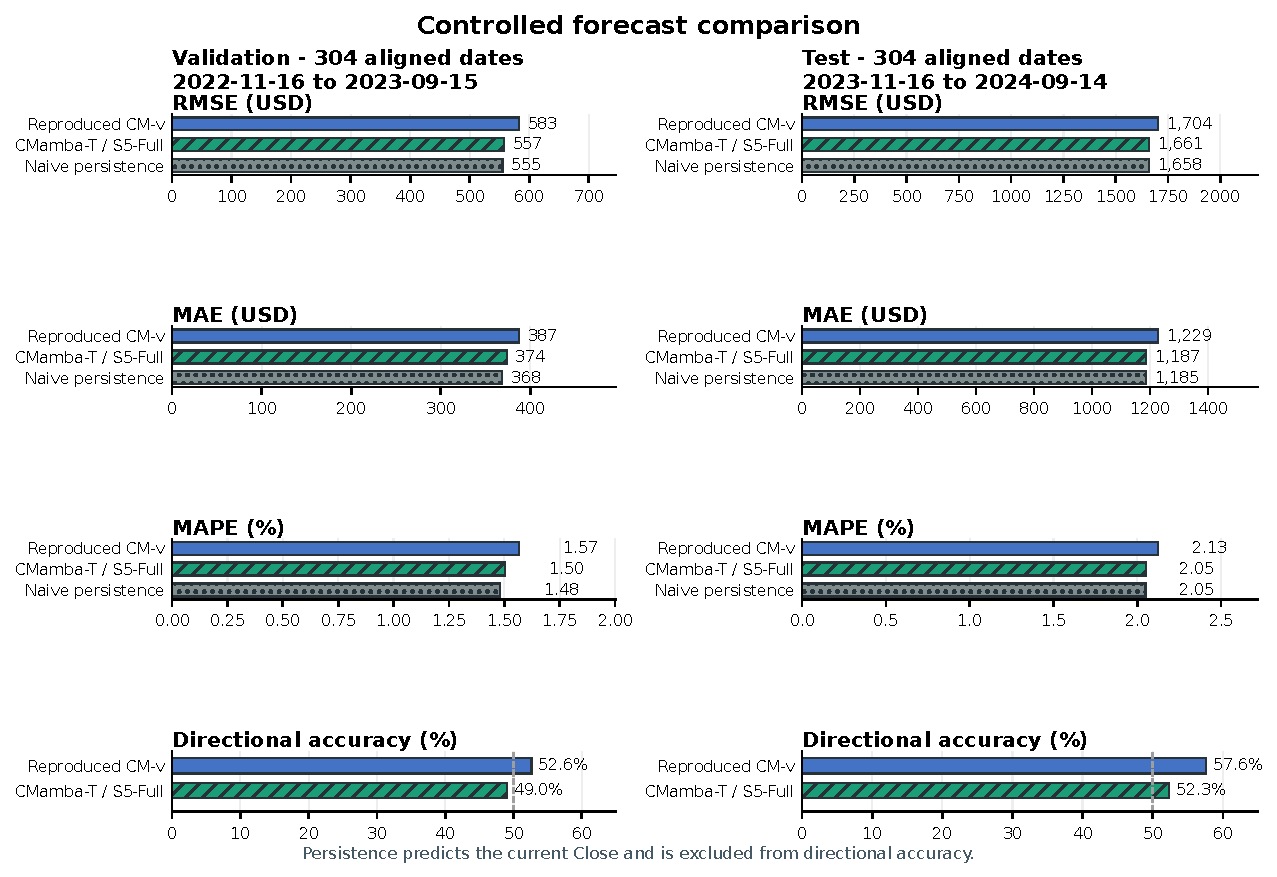
\includegraphics[width=\linewidth]{figures/controlled_forecast.pdf}
\caption[Controlled forecast comparison]{Controlled validation and test comparison on 304 aligned
target dates per split. Directional accuracy is reported only for CM-v and S5-Full.}
\label{fig:controlled-forecast}
\end{figure}

Điểm số cho thấy S5-Full thấp hơn CM-v ở cả hai split, nhưng persistence vẫn thấp hơn S5-Full. Về
hướng, CM-v cao nhất trên test. Sai số mức giá và khả năng dự đoán hướng đo hai thuộc tính khác nhau
nên cần được diễn giải riêng.

\begin{table}[H]
\centering
\caption{Khoảng tin cậy 95\% cho RMSE từ moving-block bootstrap. $\Delta$RMSE là S5-Full trừ CM-v.}
\label{tab:rmse-ci}
{\scriptsize
\begin{tabular}{@{}lrrrr@{}}
\toprule
\textbf{Split} & \textbf{CM-v} & \textbf{S5-Full} & \textbf{Persistence} & \textbf{$\Delta$RMSE [95\% CI]} \\
\midrule
Val & [\num{490.30}, \num{684.89}] & [\num{477.58}, \num{644.61}] & [\num{474.90}, \num{642.26}] & \num{-25.18} [\num{-55.69}, \num{6.54}] \\
Test & [\num{1480.46}, \num{1945.62}] & [\num{1420.73}, \num{1918.17}] & [\num{1419.78}, \num{1914.65}] & \num{-42.69} [\num{-114.49}, \num{23.44}] \\
\bottomrule
\end{tabular}}
\end{table}

\begin{table}[H]
\centering
\caption{Độ nhạy của khoảng cặp 95\% theo độ dài khối bootstrap. $\Delta$RMSE âm có lợi cho
S5-Full; $\Delta$Direction dương có lợi cho CM-v; pp là điểm phần trăm.}
\label{tab:block-sensitivity}
{\scriptsize
\begin{tabular}{@{}lrrr@{}}
\toprule
\textbf{Split} & \textbf{$L$} & \textbf{$\Delta$RMSE [95\% CI]} &
\textbf{$\Delta$Direction [95\% CI, pp]} \\
\midrule
Val & \num{5} & [\num{-55.80}, \num{5.95}] & [\num{-3.29}, \num{10.86}] \\
Val & \num{7} & [\num{-55.69}, \num{6.54}] & [\num{-2.96}, \num{10.86}] \\
Val & \num{14} & [\num{-53.02}, \num{4.23}] & [\num{-2.30}, \num{10.20}] \\
\midrule
Test & \num{5} & [\num{-116.46}, \num{23.53}] & [\num{-3.62}, \num{12.83}] \\
Test & \num{7} & [\num{-114.49}, \num{23.44}] & [\num{-3.29}, \num{12.50}] \\
Test & \num{14} & [\num{-106.55}, \num{16.23}] & [\num{-2.63}, \num{11.51}] \\
\bottomrule
\end{tabular}}
\end{table}

Mọi khoảng trong Bảng~\ref{tab:block-sensitivity} đều chứa 0. Vì vậy, kết luận cặp không thay đổi
tại $L=\num{5},\num{7},\num{14}$: chưa xác nhận được ưu thế RMSE hoặc directional accuracy của một
mô hình. Đây là kiểm tra độ nhạy giới hạn trên ba giả định phụ thuộc, không phải kết luận cho mọi độ
dài khối.

RMSE phạt độ lớn sai số, còn directional accuracy chỉ so sánh dấu thay đổi. Trên test, trung vị
độ lớn return dự báo là \num{0.67}\% cho CM-v và \num{0.12}\% cho S5-Full; S5-Full bám sát mức giá
hiện tại hơn nên có thể giảm sai số bình phương mà không cải thiện hướng. Trên validation, khoảng
95\% của directional accuracy là [\num{47.37}, \num{59.21}]\% cho CM-v và
[\num{44.41}, \num{54.28}]\% cho S5-Full; chênh lệch là \num{3.62} điểm phần trăm với khoảng
[\num{-2.96}, \num{10.86}]. Trên test, các khoảng tương ứng là
[\num{51.32}, \num{62.83}]\%, [\num{47.70}, \num{57.24}]\% và chênh lệch \num{5.26} điểm phần
trăm với khoảng [\num{-3.29}, \num{12.50}]. Cả hai khoảng chênh lệch đều chứa 0. McNemar exact
không bác bỏ giả thuyết không về tỷ lệ dự báo hướng đúng theo biên bằng nhau (validation
$p=\num{0.400}$; test $p=\num{0.224}$); kết quả này không chứng minh hai mô hình tương đương.

\begin{table}[H]
\centering
\caption{So sánh mô tả theo hai nửa thời gian; mỗi giai đoạn có 152 ngày liên tiếp.}
\label{tab:temporal-stability}
{\scriptsize
\begin{tabular}{@{}lrrrrr@{}}
\toprule
\textbf{Giai đoạn} & \textbf{CM-v RMSE} & \textbf{S5 RMSE} & \textbf{Persistence RMSE} & \textbf{CM-v Dir. (\%)} & \textbf{S5 Dir. (\%)} \\
\midrule
Val H1 & \num{599.05} & \num{561.60} & \num{559.57} & \num{50.66} & \num{48.68} \\
Val H2 & \num{565.49} & \num{553.04} & \num{550.27} & \num{54.61} & \num{49.34} \\
Test H1 & \num{1693.50} & \num{1669.26} & \num{1672.69} & \num{59.21} & \num{53.29} \\
Test H2 & \num{1713.47} & \num{1652.35} & \num{1642.26} & \num{55.92} & \num{51.32} \\
\bottomrule
\end{tabular}}
\end{table}

Val H1/H2 lần lượt là 16-11-2022--16-04-2023 và 17-04-2023--15-09-2023; Test H1/H2 là
16-11-2023--15-04-2024 và 16-04-2024--14-09-2024. S5-Full có RMSE thấp hơn CM-v ở cả bốn giai
đoạn, nhưng persistence thấp hơn S5-Full ở ba giai đoạn; CM-v có directional accuracy cao hơn ở cả
bốn. Đây là kiểm tra mô tả trên cùng checkpoint và không phải bốn lần huấn luyện hay bốn holdout độc
lập.

\begin{table}[H]
\centering
\caption{Kiểm định cặp trên 304 ngày chung. DM dùng squared error và HAC lag 1; Wilcoxon dùng
absolute error.}
\label{tab:paired-tests}
{\small
\begin{tabularx}{\linewidth}{@{}llrrll@{}}
\toprule
\textbf{Split} & \textbf{So sánh A vs B} & \textbf{DM $p$} & \textbf{Wilcoxon $p$} & \textbf{MSE thấp hơn} & \textbf{MAE thấp hơn} \\
\midrule
Val & CM-v vs persistence & \num{0.106} & \textbf{\num{0.024}} & persistence & persistence \\
Val & S5-Full vs persistence & \num{0.161} & \textbf{\num{0.017}} & persistence & persistence \\
Val & S5-Full vs CM-v & \num{0.128} & \num{0.094} & S5-Full & S5-Full \\
\midrule
Test & CM-v vs persistence & \num{0.188} & \num{0.096} & persistence & persistence \\
Test & S5-Full vs persistence & \num{0.455} & \num{0.977} & persistence & persistence \\
Test & S5-Full vs CM-v & \num{0.224} & \num{0.117} & S5-Full & S5-Full \\
\bottomrule
\end{tabularx}}
\end{table}

Trên validation, Wilcoxon cho thấy persistence có sai số tuyệt đối thấp hơn CM-v
($p=\num{0.024}$) và S5-Full ($p=\num{0.017}$); DM không bác bỏ giả thuyết độ chính xác bình phương
bằng nhau. Trên test, cả sáu giá trị $p$ đều lớn hơn 0.05. Do đó điểm RMSE thấp hơn của S5-Full so
với CM-v là kết quả quan sát được, chưa phải bằng chứng về ưu thế thống kê.

\section{RQ3: paper replay và corrected self-financing}\label{sec:rq3-results}
Bảng~\ref{tab:paper-replay} giữ nguyên giao thức giao dịch không phí của bài báo. Checkpoint chính
thức tái tạo gần như chính xác ba hàng test đã công bố. Checkpoint tái lập tạo chuỗi hành động khác,
vì vậy số dư thấp hơn dù sai số dự báo tổng hợp chỉ chênh nhẹ.

\begin{table}[htbp]
\centering
\caption{Paper replay trên test, vốn đầu \$100 và phí 0.}
\label{tab:paper-replay}
{\small
\begin{tabularx}{\linewidth}{@{}llrrrr@{}}
\toprule
\textbf{Checkpoint} & \textbf{Chiến lược} & \textbf{Paper balance} & \textbf{Local balance} & \textbf{Paper MDD (\%)} & \textbf{Local MDD (\%)} \\
\midrule
Chính thức & Vanilla & \num{246.58} & \num{246.58} & \num{23.48} & \num{23.48} \\
Chính thức & Smart & \num{213.20} & \num{213.20} & \num{13.37} & \num{13.37} \\
Chính thức & Extended Smart & \num{262.78} & \num{262.78} & \num{11.09} & \num{11.09} \\
\midrule
Tái lập & Vanilla & \num{246.58} & \num{174.94} & \num{23.48} & \num{23.94} \\
Tái lập & Smart & \num{213.20} & \num{165.25} & \num{13.37} & \num{10.20} \\
Tái lập & Extended Smart & \num{262.78} & \num{204.26} & \num{11.09} & \num{11.74} \\
\bottomrule
\end{tabularx}}
\end{table}

Bảng~\ref{tab:corrected-trading} là một bề mặt khác: 304 ngày chung, engine self-financing và phí
0.2\%. Không nên so trực tiếp số dư của bảng này với Bảng~\ref{tab:paper-replay}, vì tập ngày và quy
tắc kế toán khác nhau.

\begin{table}[htbp]
\centering
\caption{Corrected self-financing trên test, phí 0.2\%, vốn đầu \$100. Turnover và phí tính theo
USD; mọi reconciliation error bằng 0.}
\label{tab:corrected-trading}
{\scriptsize
\begin{tabularx}{\linewidth}{@{}Xlrrrrrr@{}}
\toprule
\textbf{Mô hình} & \textbf{Chiến lược} & \textbf{Final} & \textbf{ROI (\%)} & \textbf{MDD (\%)} & \textbf{Lệnh} & \textbf{Turnover} & \textbf{Phí} \\
\midrule
Đối chứng chung & Buy-and-hold & \textbf{\num{158.09}} & \textbf{\num{58.09}} & \num{26.18} & \num{1} & \num{99.80} & \num{0.20} \\
\midrule
CM-v tái lập & Vanilla & \num{115.97} & \num{15.97} & \num{26.29} & \num{46} & \num{5731.07} & \num{11.46} \\
CM-v tái lập & Smart & \num{95.92} & \num{-4.08} & \num{18.08} & \num{222} & \num{7758.47} & \num{15.52} \\
CM-v tái lập & Extended Smart & \num{92.11} & \num{-7.89} & \num{19.81} & \num{304} & \num{19450.28} & \num{38.90} \\
\midrule
S5-Full & Vanilla & \num{100.00} & \num{0.00} & \num{0.00} & \num{0} & \num{0.00} & \num{0.00} \\
S5-Full & Smart & \num{103.08} & \num{3.08} & \num{1.91} & \num{133} & \num{124.35} & \num{0.25} \\
S5-Full & Extended Smart & \num{98.39} & \num{-1.61} & \num{5.00} & \num{304} & \num{508.33} & \num{1.02} \\
\midrule
Persistence & Cả ba chế độ & \num{100.00} & \num{0.00} & \num{0.00} & \num{0} & \num{0.00} & \num{0.00} \\
\bottomrule
\end{tabularx}}
\end{table}

\begin{figure}[htbp]
\centering
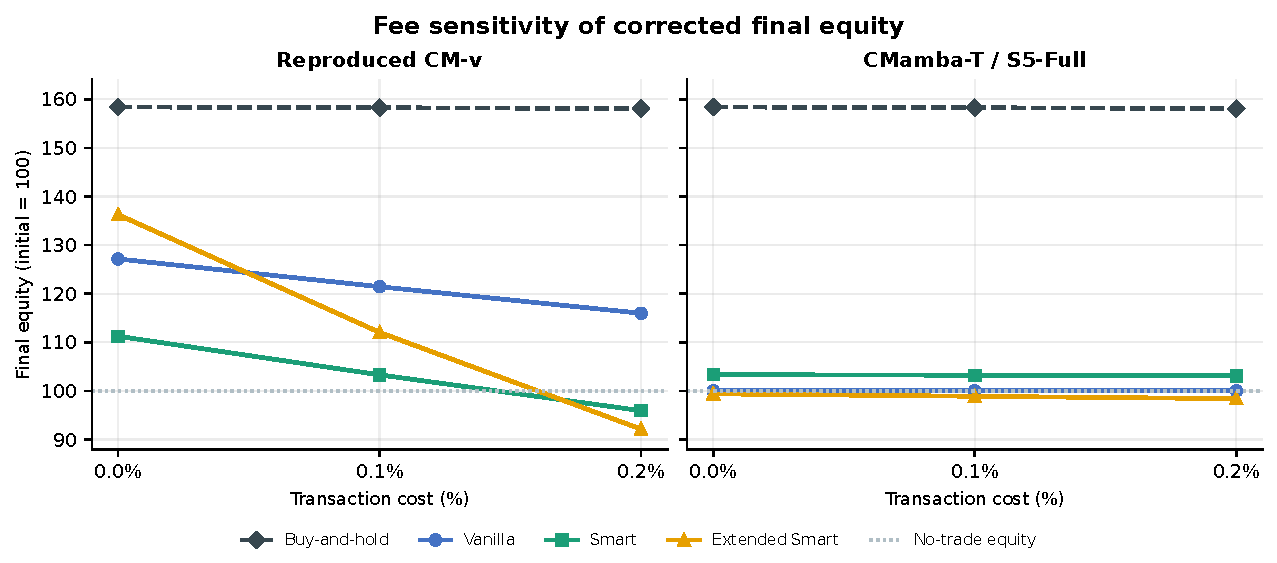
\includegraphics[width=\linewidth]{figures/corrected_trading.pdf}
\caption[Fee sensitivity of corrected final equity]{Fee sensitivity of corrected final equity on
the 304-date test split. Each panel compares Buy-and-hold, Vanilla, Smart and Extended Smart at
0\%, 0.1\% and 0.2\% transaction cost.}
\label{fig:corrected-trading}
\end{figure}

Không chiến lược forecast-driven nào vượt buy-and-hold ở bất kỳ mức phí nào. Khi phí tăng từ 0\% lên
0.2\%, CM-v Vanilla giảm từ \num{127.14} xuống \num{115.97}, Smart từ \num{111.23} xuống
\num{95.92}, và Extended Smart từ \num{136.25} xuống \num{92.11}. S5-Full Smart chỉ giảm từ
\num{103.34} xuống \num{103.08}; Vanilla không phát lệnh. Vì vậy kết luận RQ3 không phụ thuộc riêng
vào mức 0.2\%: paper replay tái tạo thuật toán công bố, còn corrected engine không xác nhận ưu thế
kinh tế; policy có turnover cao nhạy với phí hơn.

% ---------------------------------------------------------------------
\chapter{Thử nghiệm CMamba-T/S5-Full}\label{chap:s5}

\section{Thiết kế và quy mô}\label{sec:s5-design}
CM-v chính thức và CM-v tái lập đều giữ tensor $[B,6,14]$ của bài báo. Trong một thí nghiệm cục bộ
tách biệt, S5-Full nhận chuỗi 60 day-token có embedding 32 chiều. Cửa sổ dài và độ rộng mô hình trở
thành hai đại lượng độc lập; đây là khác biệt cấu trúc có thể xác nhận từ mã nguồn. Thí nghiệm thay
đổi đồng thời cửa sổ đầu vào, tiền xử lý, cách tham số hoá đầu ra và kiến trúc, nên không phải một
ablation chỉ thay đổi kiến trúc.

S5-Full có \num{57249} tham số, bằng \num{41.80}\% CM-v và giảm \num{58.20}\%. Hình
\ref{fig:params-error} đặt quy mô này cạnh RMSE trên cùng các split; persistence là đường tham chiếu
0 tham số, không phải một điểm mô hình học được.

\begin{figure}[htbp]
\centering
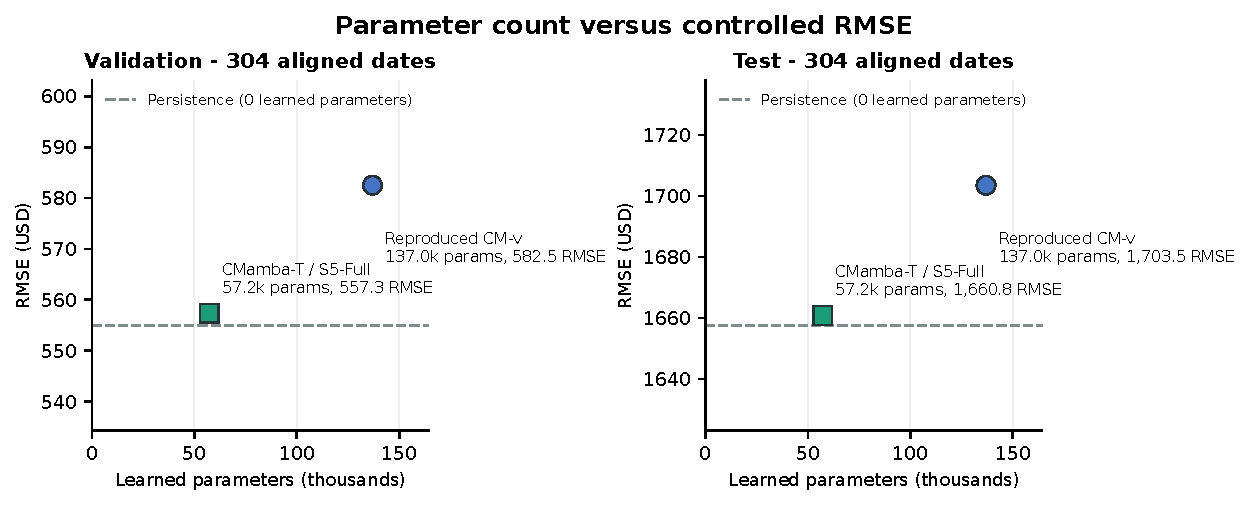
\includegraphics[width=\linewidth]{figures/params_vs_error.pdf}
\caption[Parameter count versus forecast error]{Parameter count versus validation and test RMSE.
Only CM-v and S5-Full are learned models; persistence is a zero-parameter reference.}
\label{fig:params-error}
\end{figure}

\section{Kết quả dự báo và giao dịch}\label{sec:s5-results}
Trên validation, S5-Full giảm RMSE \num{25.18} so với CM-v (\num{557.34} so với \num{582.52}) nhưng
cao hơn persistence \num{2.40}. Trên test, S5-Full giảm RMSE \num{42.69} so với CM-v
(\num{1660.83} so với \num{1703.51}) nhưng cao hơn persistence \num{3.28}. So sánh S5-Full với
CM-v không có ý nghĩa ở DM hoặc Wilcoxon trên cả validation và test
(Bảng~\ref{tab:paired-tests}).

Trong corrected trading, S5-Full Smart kết thúc từ \$\num{103.34} đến \$\num{103.08} khi phí tăng
từ 0\% lên 0.2\%; Vanilla không phát lệnh và Extended Smart kết thúc ở \$\num{98.39} tại 0.2\%.
Kết quả này cho thấy forecast error thấp hơn CM-v không đồng nghĩa với lợi nhuận cao hơn trong mọi
policy.

\section{Kết luận cho RQ4}\label{sec:s5-conclusion}
S5-Full có RMSE điểm thấp hơn CM-v tái lập trên validation và test nhưng không thấp hơn persistence.
Các kiểm định cặp và khoảng tin cậy không xác nhận ưu thế tổng quát. Chỉ checkpoint seed 23 được đánh
giá; mọi kết quả chỉ đặc trưng cho lần huấn luyện này, không phản ánh biến thiên giữa các lần huấn
luyện.

% ---------------------------------------------------------------------
\chapter{Hệ thống minh hoạ}\label{chap:system}

\section{Kiến trúc và luồng chính}\label{sec:system-flow}
Hệ thống gồm frontend React/TypeScript, backend FastAPI và worker Python của repo lõi. Backend phục vụ
các bảng đánh giá và chuyển yêu cầu dự báo tới worker để chạy checkpoint đã chọn. Dữ liệu không hợp
lệ hoặc checkpoint không khả dụng được trả về dưới dạng lỗi, không thay thế bằng kết quả mô phỏng.

\begin{figure}[htbp]
\centering
\resizebox{\linewidth}{!}{% Primary prediction path with separate analysis and presentation outputs.
\begingroup
\definecolor{flowBlue}{HTML}{E8F0FB}
\definecolor{flowBlueEdge}{HTML}{5A7FBE}
\definecolor{flowGreen}{HTML}{E4F3EC}
\definecolor{flowGreenEdge}{HTML}{418B72}
\definecolor{flowGold}{HTML}{FFF1CF}
\definecolor{flowGoldEdge}{HTML}{B4882C}
\definecolor{flowViolet}{HTML}{F0EAF8}
\definecolor{flowVioletEdge}{HTML}{8068A6}
\definecolor{flowGrey}{HTML}{F5F7F9}
\definecolor{flowGreyEdge}{HTML}{AAB4BD}
\definecolor{flowInk}{HTML}{263238}

\tikzset{
  input/.style={draw=flowBlueEdge, fill=flowBlue, rounded corners=3pt,
    minimum width=1.9cm, minimum height=1.05cm, align=center, inner sep=4pt,
    font=\sffamily\small\bfseries, text=flowInk},
  process/.style={draw=flowGreenEdge, fill=flowGreen, rounded corners=3pt,
    minimum width=2.25cm, minimum height=1.05cm, align=center, inner sep=4pt,
    font=\sffamily\small\bfseries, text=flowInk},
  repeat/.style={draw=flowVioletEdge, fill=flowViolet, rounded corners=3pt,
    minimum width=2.25cm, minimum height=1.05cm, align=center, inner sep=4pt,
    font=\sffamily\small\bfseries, text=flowInk},
  head/.style={draw=flowGoldEdge, fill=flowGold, rounded corners=3pt,
    minimum width=2.25cm, minimum height=1.05cm, align=center, inner sep=4pt,
    font=\sffamily\small\bfseries, text=flowInk},
  output/.style={draw=flowBlueEdge, fill=flowBlue, rounded corners=3pt,
    minimum width=2.1cm, minimum height=1.05cm, align=center, inner sep=4pt,
    font=\sffamily\small\bfseries, text=flowInk},
  group/.style={draw=flowGreyEdge, fill=flowGrey, dashed, rounded corners=6pt,
    line width=0.75pt, inner xsep=7pt, inner ysep=8pt},
  note/.style={font=\sffamily\small\bfseries, text=flowInk, align=left},
  flow/.style={-{Stealth[scale=1.2]}, draw=flowInk, line width=0.85pt},
  junction/.style={circle, draw=flowInk, fill=flowInk, minimum size=3.2pt,
    inner sep=0pt}
}

\begin{tikzpicture}[font=\sffamily\small, node distance=0.6cm and 0.8cm]
  \node[input] (data)
    {OHLCV\\data\\{\scriptsize\mdseries CSV / paper split}};
  \node[process, right=of data] (validate)
    {Validate and\\preprocess\\{\scriptsize\mdseries schema + causal order}};
  \node[process, right=of validate] (select)
    {Select model/\\window\\{\scriptsize\mdseries CM-v: 14; S5-Full: 60}};
  \node[head, right=of select] (inference)
    {Local checkpoint\\inference};
  \node[output, right=of inference] (forecast)
    {Next-day\\forecast};

  \node[note, above=0.34cm of data.north west, anchor=south west] (predictionTitle)
    {Prediction workflow};

  \draw[flow] (data) -- (validate);
  \draw[flow] (validate) -- (select);
  \draw[flow] (select) -- (inference);
  \draw[flow] (inference) -- (forecast);

  \node[junction, below=1.70cm of inference] (analysisHub) {};
  \node[repeat, below=0.65cm of analysisHub] (replay)
    {Historical\\replay\\{\scriptsize\mdseries paper protocol}};
  \node[repeat, left=of replay] (evaluation)
    {Forecast\\evaluation\\{\scriptsize\mdseries common dates + paired tests}};
  \node[repeat, right=of replay] (trading)
    {Corrected\\trading\\{\scriptsize\mdseries self-financing + costs}};
  \node[output, below=of replay] (console)
    {Five-screen\\Console};

  \node[note, above=0.24cm of analysisHub] (analysisTitle)
    {Analysis and presentation};

  \draw[flow] (forecast.south) |- (analysisHub.east);
  \draw[flow] (analysisHub) -- (evaluation.north);
  \draw[flow] (analysisHub) -- (replay.north);
  \draw[flow] (analysisHub) -- (trading.north);
  \draw[flow] (evaluation.south) |- (console.west);
  \draw[flow] (replay) -- (console);
  \draw[flow] (trading.south) |- (console.east);

  \begin{scope}[on background layer]
    \node[group, fit=(predictionTitle)(data)(validate)(select)(inference)(forecast)] {};
    \node[group,
      fit=(analysisTitle)(analysisHub)(evaluation)(replay)(trading)(console)] {};
  \end{scope}
\end{tikzpicture}
\endgroup
}
\caption[System workflow]{Primary workflow from OHLCV validation and local checkpoint inference to
forecast evaluation, historical replay, corrected trading, and the five-screen Console.}
\label{fig:system-flow}
\end{figure}

Luồng chính là upload/paper dataset $\to$ chọn CM-v hoặc S5-Full $\to$ chạy \emph{local checkpoint}
$\to$ hiển thị dự báo, return kỳ vọng và cửa sổ đầu vào. CM-v yêu cầu ít nhất 14 nến;
S5-Full yêu cầu 60 nến. Historical replay là chế độ độc lập. Live HTTP nằm trong phần nâng cao và
chỉ gửi request khi người dùng chủ động chạy.

\section{Năm màn hình}\label{sec:five-screens}
Console giữ đúng kiến trúc \emph{five-screen}; nội dung trên giao diện và trong hình đều bằng tiếng
Anh. Bảng~\ref{tab:screens} ánh xạ từng màn hình tới vai trò trong luận văn.

\begin{table}[htbp]
\centering
\caption{Vai trò của năm màn hình Console.}
\label{tab:screens}
\begin{tabularx}{\linewidth}{@{}lXX@{}}
\toprule
\textbf{Màn hình} & \textbf{Chức năng} & \textbf{Kết quả hiển thị} \\
\midrule
Data & Nạp CSV, kiểm tra schema, thứ tự, giá trị và lịch sử & OHLCV đã xác thực \\
Evaluation & So sánh số liệu công bố, kết quả cục bộ và kiểm định cặp & Chỉ số dự báo \\
Predict & Chọn checkpoint, dự báo dữ liệu bài báo hoặc dữ liệu mới; replay tách riêng & Giá ngày kế tiếp \\
Trading & Chuyển giữa paper replay và corrected self-financing & Hai trading protocols \\
Architecture & So sánh mô tả bài báo, đường chạy CM-v và S5-Full & Kiến trúc mô hình \\
\bottomrule
\end{tabularx}
\end{table}

\begin{figure}[p]
\centering
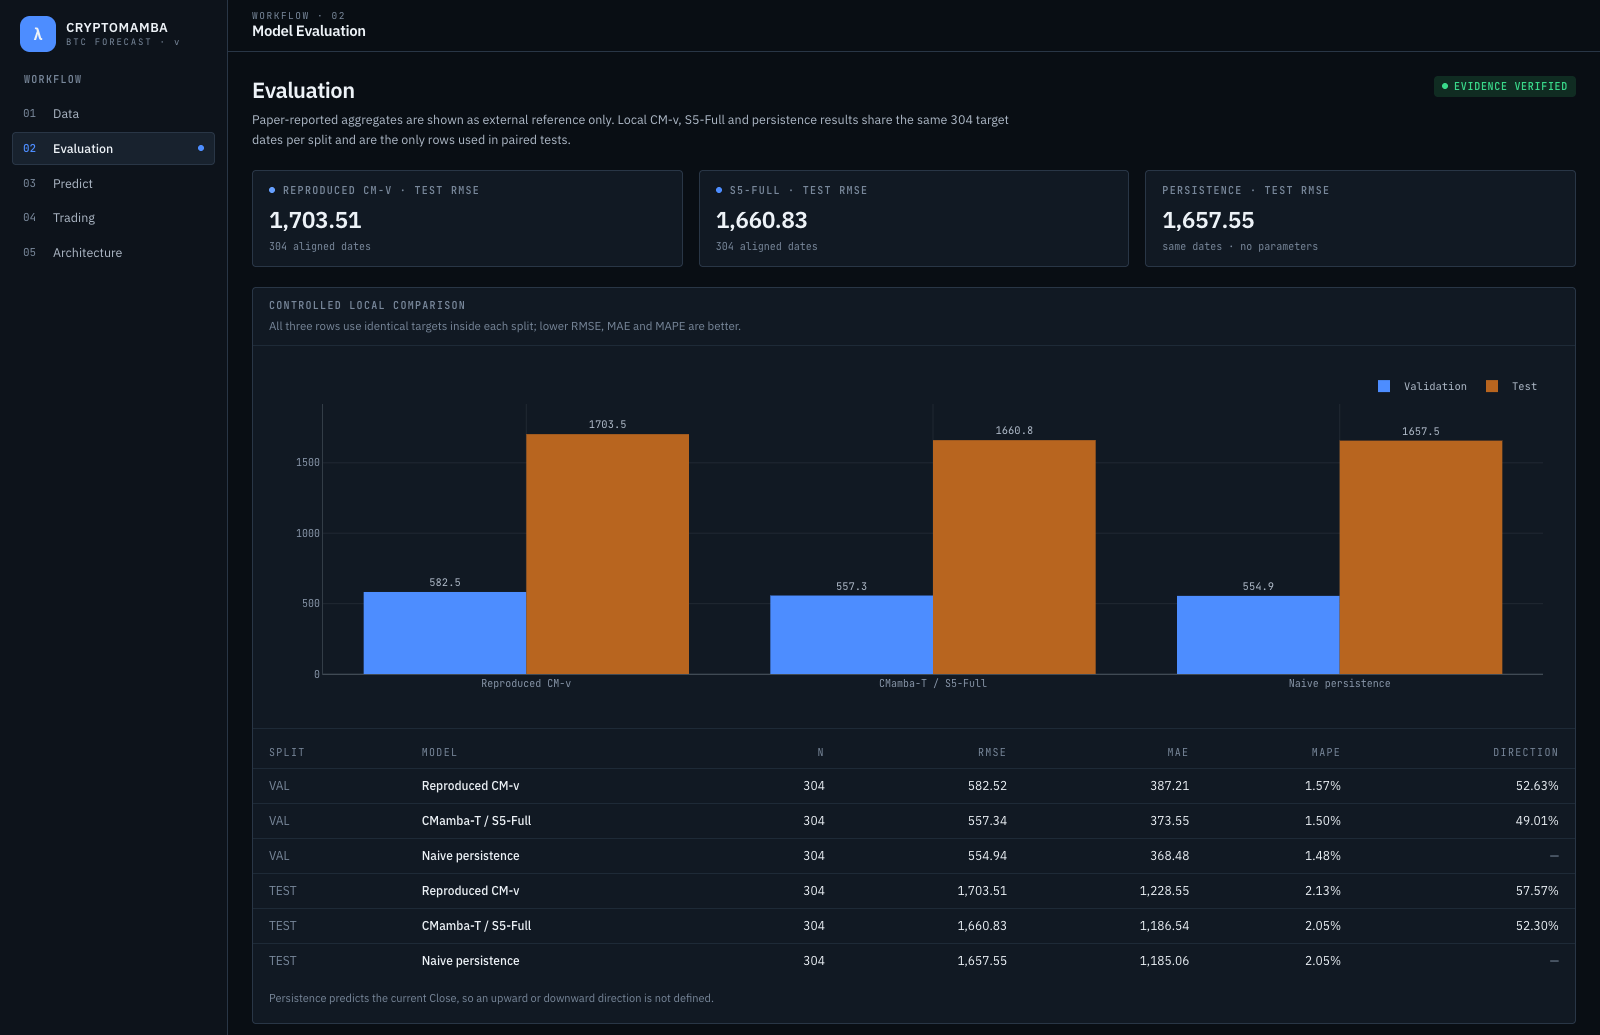
\includegraphics[width=\linewidth]{figures/ui/ui_evaluation.png}
\caption[Evaluation screen]{Evaluation screen: controlled validation/test RMSE and the aligned
local metric table.}
\label{fig:ui-evaluation}
\end{figure}

\begin{figure}[p]
\centering
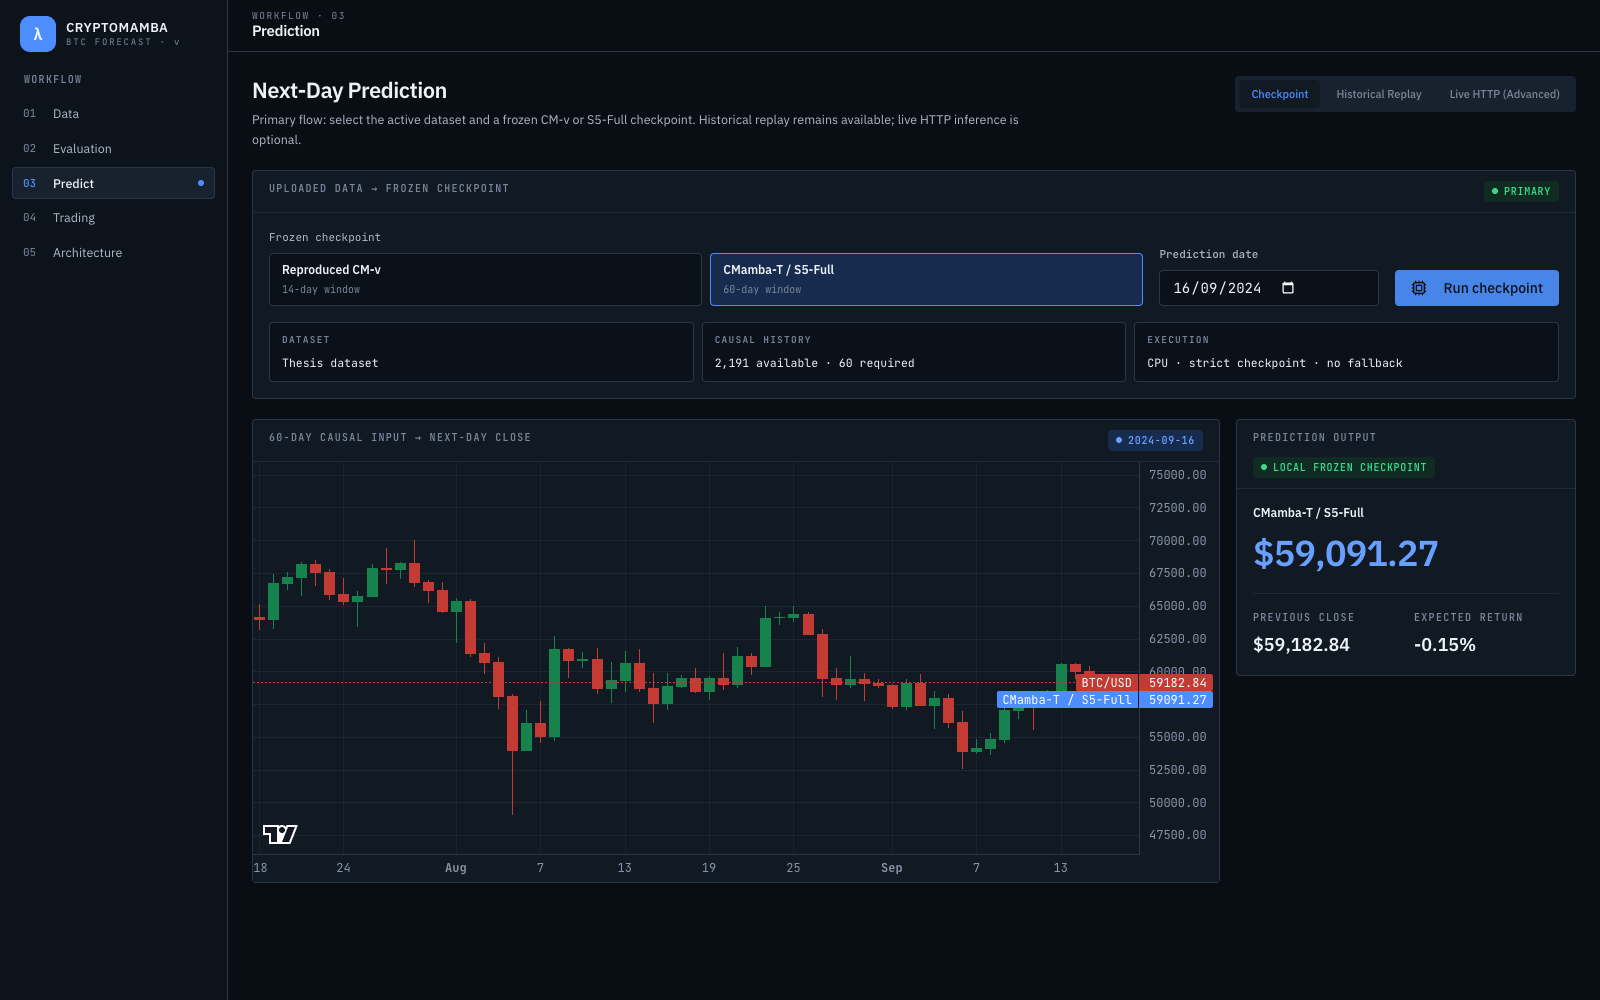
\includegraphics[width=\linewidth]{figures/ui/ui_predict.png}
\caption[Predict screen]{Predict screen: uploaded or paper data is sent to the selected CM-v or
S5-Full local checkpoint; the model window remains visible.}
\label{fig:ui-predict}
\end{figure}

\begin{figure}[p]
\centering
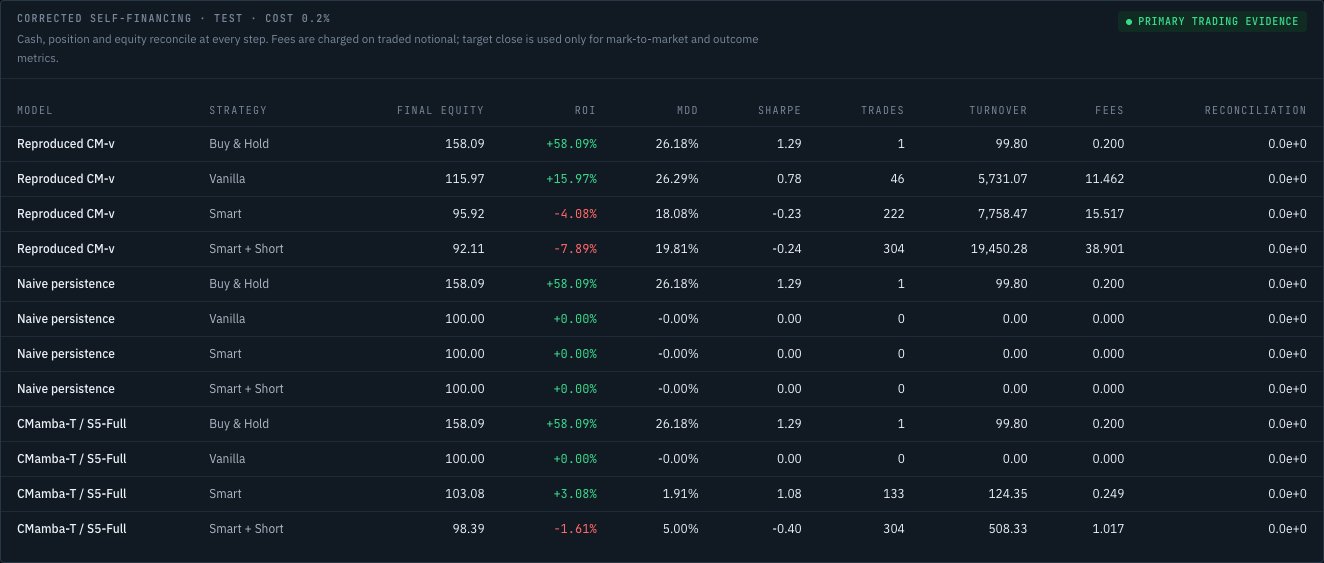
\includegraphics[width=\linewidth]{figures/ui/ui_trading.png}
\caption[Trading screen]{Trading screen: the corrected self-financing result is shown separately
from the original paper replay.}
\label{fig:ui-trading}
\end{figure}

\section{Kiểm tra chức năng}\label{sec:system-validation}
Kiểm tra tự động bao phủ parsing CSV, giới hạn cửa sổ, suy luận bằng hai mô hình, dữ liệu không hợp lệ
và các bất biến kế toán. Kiểm tra trình duyệt đi qua cả năm màn hình, hai checkpoint, CSV hợp lệ và
không hợp lệ, lịch sử ngắn hơn 60 ngày, historical replay và hai giao thức giao dịch. Các phép kiểm
tra này xác nhận chức năng của prototype; luận văn không kết luận về usability khi chưa có nghiên cứu
người dùng.

% ---------------------------------------------------------------------
\chapter{Bàn luận và kết luận}\label{chap:discussion}

\section{Trả lời các câu hỏi nghiên cứu}\label{sec:answers}
\textbf{RQ1.} Checkpoint chính thức tái tạo gần như chính xác dự báo và paper trading replay. Trên
350 ngày, checkpoint tái lập chênh \num{0.892}\% RMSE, \num{1.057}\% MAE và \num{0.718}\% MAPE so
với kết quả công bố.

\textbf{RQ2.} Trên 304 ngày chung, persistence có RMSE thấp nhất ở cả validation và test. S5-Full
thấp hơn CM-v về điểm RMSE ở cả bốn nửa thời gian, nhưng khoảng chênh lệch bootstrap chứa 0 và DM
không xác nhận khác biệt. CM-v có directional accuracy cao hơn, song khoảng chênh lệch và McNemar
không xác nhận ưu thế theo cặp. Các kết luận này không đổi với độ dài khối bootstrap \num{5},
\num{7} và \num{14}. Sai số mức giá và hướng đo hai thuộc tính khác nhau.

\textbf{RQ3.} Paper replay xác nhận khả năng tái tạo thuật toán công bố. Với engine self-financing,
không chiến lược dựa trên dự báo nào vượt buy-and-hold ở phí 0\%, 0.1\% hoặc 0.2\% trên cùng 304 ngày
test. Turnover giải thích mức nhạy phí của các policy giao dịch dày.

\textbf{RQ4.} S5-Full giảm \num{58.20}\% tham số và có RMSE thấp hơn CM-v trên hai split được đo,
nhưng không vượt persistence. Đóng góp mô hình vì vậy là một thí nghiệm nhẹ được đánh giá trên cả
dự báo, kiểm định và giao dịch, không phải kết luận về mô hình tốt nhất.

\section{Giới hạn}\label{sec:limitations}
\begin{itemize}
\item Dữ liệu chỉ gồm một tài sản, một tần suất và một horizon; thứ hạng không tự mở rộng sang tài
sản hoặc giai đoạn khác.
\item Cửa sổ 60 ngày của S5-Full chưa được so sánh với các lựa chọn khác. Test lịch sử đã được dùng
để báo cáo, nên quyết định tiếp theo cần một holdout mới.
\item Corrected engine giữ quy ước khớp lệnh tại Close ngày tín hiệu để đối chiếu. Đây là một trừu
tượng same-close; đánh giá thực tế cần next-open execution, slippage, spread và borrow cost quan sát.
\item Console là prototype cục bộ. Chưa có kiểm thử tải, kiểm toán bảo mật triển khai, nghiên cứu
người dùng hoặc kết nối tới hệ thống đặt lệnh.
\end{itemize}

\section{Hướng phát triển}\label{sec:future}
Ưu tiên nghiên cứu là đóng băng giao thức hiện tại và đánh giá một lần trên holdout sau tháng
09-2024, sau đó lặp nhiều seed và so sánh cửa sổ theo một giao thức validation cố định. Các mở rộng
tiếp theo có thể thêm dữ liệu ngoại sinh,
đa tài sản và horizon khác; trading engine nên chuyển sang next-open execution với mô hình chi phí
đầy đủ. Live HTTP có thể được triển khai như một adapter tuỳ chọn sau khi hoàn thành xác thực vận
hành; nó không thay đổi contract checkpoint cục bộ.

\newpage
\section{Kết luận}\label{sec:conclusion}
Luận văn không chỉ lặp lại một bảng kết quả đã công bố. Nó tách rõ số liệu Paper-reported và kết quả
cục bộ, căn mọi so sánh trên cùng ngày, bổ sung persistence cùng kiểm định cặp, đối chiếu paper replay
và xây dựng corrected backtest có thể đối soát. S5-Full mở rộng phạm vi từ tái lập sang thí nghiệm
mô hình nhẹ, nhưng kết luận được giới hạn đúng bởi persistence và ý nghĩa thống kê. Console năm màn
hình đưa toàn bộ chuỗi data--prediction--evaluation--trading--architecture lên một bề mặt có thể
kiểm tra trực tiếp từ checkpoint.

Trong bối cảnh thị trường tài sản mã hóa đang được thí điểm tại Việt Nam, giá trị ứng dụng của
prototype nằm ở khả năng minh hoạ quy trình và giới hạn thực nghiệm, không phải ở việc phát tín hiệu
đầu tư.

% ---------------------------------------------------------------------
\section*{Tính khả dụng của dữ liệu và mã nguồn}\label{sec:availability}
\addcontentsline{toc}{section}{Tính khả dụng của dữ liệu và mã nguồn}

Bài báo và mã nguồn gốc có tại \url{https://arxiv.org/abs/2501.01010} và
\url{https://github.com/MShahabSepehri/CryptoMamba}. Dữ liệu dự báo, kiểm định và giao dịch dùng cho
các bảng kết quả được cung cấp cùng tài liệu dự án.

% ---------------------------------------------------------------------
\begin{thebibliography}{99}
\addcontentsline{toc}{chapter}{Tài liệu tham khảo}

\bibitem{cryptomamba}
Sepehri, M. S., Mehradfar, A., Soltanolkotabi, M., và Avestimehr, S.
\textit{CryptoMamba: Leveraging State Space Models for Accurate Bitcoin Price Prediction}.
IEEE ICBC, 2025; arXiv:2501.01010v2. \url{https://arxiv.org/abs/2501.01010}.

\bibitem{mamba}
Gu, A. và Dao, T. \textit{Mamba: Linear-Time Sequence Modeling with Selective State Spaces}.
arXiv:2312.00752, 2023. \url{https://arxiv.org/abs/2312.00752}.

\bibitem{itransformer}
Liu, Y. và cộng sự. \textit{iTransformer: Inverted Transformers Are Effective for Time Series
Forecasting}. ICLR, 2024. \url{https://openreview.net/forum?id=JePfAI8fah}.

\bibitem{smamba}
Wang, Z. và cộng sự. \textit{Is Mamba Effective for Time Series Forecasting?}
arXiv:2403.11144, 2024. \url{https://arxiv.org/abs/2403.11144}.

\bibitem{dm}
Diebold, F. X. và Mariano, R. S. \textit{Comparing Predictive Accuracy}.
Journal of Business \& Economic Statistics, 13(3), 253--263, 1995.
\url{https://doi.org/10.1080/07350015.1995.10524599}.

\bibitem{wilcoxon}
Wilcoxon, F. \textit{Individual Comparisons by Ranking Methods}.
Biometrics Bulletin, 1(6), 80--83, 1945. \url{https://doi.org/10.2307/3001968}.

\bibitem{neweywest}
Newey, W. K. và West, K. D. \textit{A Simple, Positive Semi-Definite, Heteroskedasticity and
Autocorrelation Consistent Covariance Matrix}. Econometrica, 55(3), 703--708, 1987.
\url{https://doi.org/10.2307/1913610}.

\bibitem{kunsch1989}
Künsch, H. R. \textit{The Jackknife and the Bootstrap for General Stationary Observations}.
The Annals of Statistics, 17(3), 1217--1241, 1989.
\url{https://doi.org/10.1214/aos/1176347265}.

\bibitem{buhlmann1999}
Bühlmann, P. và Künsch, H. R. \textit{Block Length Selection in the Bootstrap for Time Series}.
Computational Statistics \& Data Analysis, 31(3), 295--310, 1999.
\url{https://doi.org/10.1016/S0167-9473(99)00014-6}.

\bibitem{mcnemar1947}
McNemar, Q. \textit{Note on the Sampling Error of the Difference between Correlated Proportions or
Percentages}. Psychometrika, 12(2), 153--157, 1947.
\url{https://doi.org/10.1007/BF02295996}.

\bibitem{nq05}
Chính phủ nước Cộng hòa xã hội chủ nghĩa Việt Nam. \textit{Nghị quyết số 05/2025/NQ-CP ngày
09-09-2025 về việc triển khai thí điểm thị trường tài sản mã hóa tại Việt Nam}. 2025.
\url{https://vanban.chinhphu.vn/?pageid=27160&docid=215249}.
\end{thebibliography}

\end{document}
